\documentclass[main.tex]{subfiles}

\begin{document}
	\section{Architectural Design}
	
	\subsection{Block Diagram}
	
	SOS has a relatively traditional scanner, parser, ast, semant and codegen architecture. Then, C math library, OpenGL and Off-Screen Rendering Mesa library are added to cc compiler to compile to one executable file.
	
	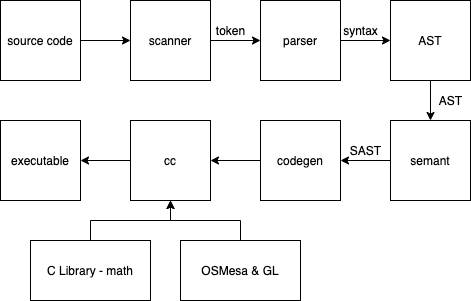
\includegraphics[width=\textwidth]{compiler_arch.png}
	
	\paragraph{sos.ml} by Sheron. The top level of our compiler, serves as one entry point for the source code to go through scanner, parser, AST, semant, codegen and then generate LLVM IR.
	
	\paragraph{scanner.mll} by Sheron and G. Receives the source code and uses OCaml Lexer to process it to tokens.
	
	\paragraph{parser.mly} by G and Sheron. Reads from scanner, generate AST from tokens. Reject when there is an error.
	
	\paragraph{AST}
	    \subparagraph{ast.mli} by G and Sheron. This file only preserves the abstract syntax tree structure.
	    \subparagraph{astprint.ml} by G. Contains helper functions to generate code from one AST and print it out. Use flag "-a" in compiler to call the function while compiling.
	    
    \paragraph{semant.ml} by G, Tojo and Sheron. Receives one AST and check if it is semantically correct. We also store the information of all external functions at the beginning of the semant to check, and pass to codegen for further use.
	
	\paragraph{SAST}
	    \subparagraph{sast.mli} by G. This file only preserves the semantically checked abstract syntax tree structure.
	    \subparagraph{sastprint.ml} by G. Contains helper functions to generate code from one SAST and print it out. Use flag "-s" in compiler to call the function while compiling.
	    
    \paragraph{Codegen.ml} by G, Sheron and Sitong. This file contains all the instructions to generate LLVM IR and call external functions from C and OpenGL libraries.
    
    \paragraph{External Functions}
        \subparagraph{util\_math.c} by Sheron. As we usually call functions of C Math library directly, there is only one function called "toradians" in this file.
        
        \subparagraph{util\_opengl.c} by Tojo, Sheron. Takes in pointers allocated in SOS and call the function such as start and stop render or draw points, path and shape. Standard libraries written in SOS provide more user friendly wrappers of these C functions. For the writing to file and canvas initialization part, we consulted the code from mesa-demos, an official collection of OpenGL / Mesa demos and test programs.
    
    \paragraph{Compile}
        \subparagraph{Makefile} by G, Sheron, Tojo and Sitong. Make, test and clean SOS native file.
        \subparagraph{Dockerfile} by Sheron. To install all dependencies for compiler and OpenGL based on Ubuntu 20.04 LTS. See next subsection for more details.
        \subparagraph{shell scripts} by G and Sheron. Those are for pulling and connecting docker image, or compiling executables.
        \subparagraph{miscellaneous tests} by Tojo. Check Test Plan section for more details.
    
    \paragraph{Standard Libraries} by G, Tojo, Sheron and Sitong. All written in pure SOS and could be imported. Extends the functionality of SOS language, and provides wrappers to external functions. See LRM for more details.
	
	\subsection{External Libraries}
	
	We link C Math Library and Mesa Library to LLVM IR code in CC compiler directly.
	
	For OpenGL, we are using The Mesa 3D Graphics Library, which is one open source software implementation. We choose Mesa because it has one off-screen rendering interface. Because it is off-screen, it renders into main memory without any sort of window system or operating system dependencies. Thus, it could run inside of a docker image provided by us smoothly. In the end, SOS writes the buffer in memory to a file when user decides to end rendering, which is more practical than window system rendering.
	
	The Dockerfile provides instructions of how to download and compile all dependencies needed in Ubuntu 20.04 LTS. Most of the dependencies could be installed by package management tools such as apt-get, pip and opam. However, we need to compile Mesa library by downloading and compiling. There are two choices to play with the docker image: compile (might cost about 1 hour on my computer) or pull(around 7 GB).
	
\end{document}